\clearpage
\section{File Format}\label{sec:file}
We use XML files to define the copter used in our design and simulation tool. A list of sample files are provided in the folder \texttt{resources/copter/} for your reference. To load an XML file, simply use its name as the first argument when you run \texttt{copter\_viewer}. For example:
\begin{verbatim}
> ./copter_viewer y6copter.xml
\end{verbatim}
will load a Y6 hexacopter defined in \texttt{y6copter.xml} (Figure~\ref{fig:y6_ui}). If no XML file is given, then \texttt{pentacopter.xml} is used by default.
\begin{figure}[htb]
	\centering
	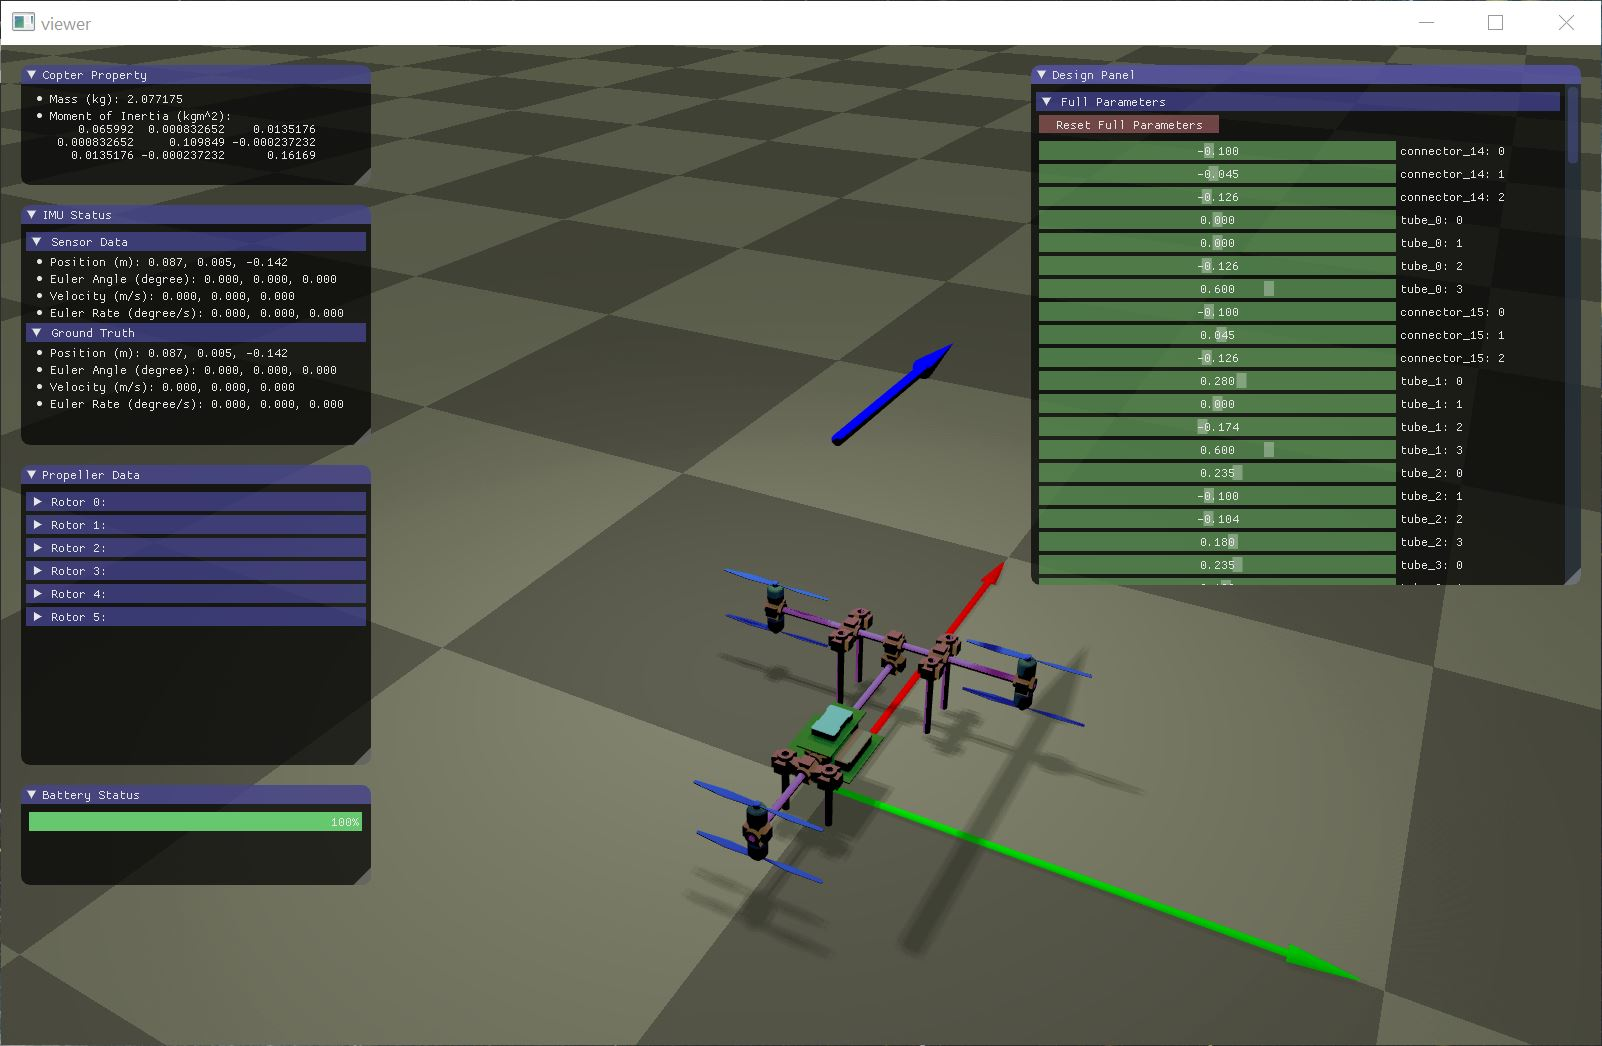
\includegraphics[width=1.0\linewidth]{y6_ui}
	\caption{Loading a Y6 hexacopter from the given XML file \texttt{y6copter.xml}.}
	\label{fig:y6_ui}
\end{figure}

The XML file itself its pretty straightforward: once you learn the rules, you are free to create your own XML files and use the software to design and simulate them. For simplicity, below we will walk you through \texttt{quadcopter.xml} so that you can get an idea of how to write your own copter file.

\subsection{Basic Structure}
The XML file starts with a line defining the version:
\begin{verbatim}
<?xml version="1.0" ?>
\end{verbatim}

The whole copter is then wrapped by a pair of tags \texttt{<copter>} and \texttt{</copter>}. You should put all your components inside these opening and closing tags. To define a complete copter, you will have to provide definitions for the following components: plates, a battery, an electronic device, tubes, connectors, propellers, and motors. All meshes used here must be watertight, otherwise we won't be able to estimate their moment of inertia.

\subsection{3D Transforms}
Many of the components are defined in their own frames in the mesh file. To place them correctly you need to apply a series of transforms. In the XML file you can specify it by using \texttt{translate} and \texttt{rotate} tags. Scaling is in general not supported except for plates and tubes.

To apply a translation, use the following tag:
\begin{verbatim}
<translate xyz="0 1 2"/>
\end{verbatim}
Applying it will move the mesh by $(0,1,2)$.

Rotation is defined by Euler angles $(\phi,\theta,\psi)$, which are also known as roll, pitch and yaw. We first rotate the mesh along its own $z$ axis by $\psi$, then around its own (new) $y$ axis by $\theta$, finally along its (new) $x$ axis by $\phi$. The angles are in degrees and its sign is defined by the right-hand rule.
\begin{verbatim}
<rotate xyz="0 0 90"/>
\end{verbatim}
In this example, we rotate the mesh by 90 degrees around its own $z$ axis.

You can apply a series of translation/rotation to a single mesh. For example, if you want to translate it first by $(0, 1, 2)$, then rotate it by $(45, 0, 90)$, then translate it by $(3, 4, 5)$:
\begin{verbatim}
<translate xyz="0 1 2"/>
<rotate rpy="45 0 90"/>
<translate xyz="3 4 5"/>
\end{verbatim}

We will see many 3D transform examples shortly.

Finally, the world frame in which we define the copter is NED (north east down), which means \textbf{negative} $z$ is the \textbf{up} direction. To avoid penetrating the ground, we usually lift our copter a little in the definition.

\subsection{Add Plates}
To define a plate, you will need to first create the tag \texttt{<plate>} and \texttt{</plate>} with two attributes: \texttt{file} specifies the mesh file, and \texttt{density} defines its density:
\begin{verbatim}
<plate file="plate.obj" density="1180.0">
  ...
</plate>
\end{verbatim}
In our code, we look for a file named \texttt{plate.obj} in the folder \texttt{resources/mesh}, which we have provided along with the source code. This mesh is a 1m$\times$1m$\times$0.0024m axis-aligned cuboid centered at the origin, and the unit of the density value is kg$/$m$^3$.

Between \texttt{<plate>} and \texttt{</plate>} you can create multiple plates by using \texttt{<instance>} tag, one for each plate. An \texttt{<instance>} tag needs you to specify the size of your plate along $x$ and $y$ direction first, then specify the location and orientation of the plate by applying translation or rotation.
\begin{verbatim}
<instance size="0.15 0.15">
  <translate xyz="0 0 -0.1"/>
</instance>
\end{verbatim}
Here we define our first plate: it is a $0.15$m$\times0.15$m$\times0.0024$m cuboid, and it is lifted by $0.1$ meters. The second plate has a smaller size ($0.15$m$\times0.07$m), and it is lifted by $0.148$ meters, leaving a $0.048-0.0024=0.0456$ meters gap between them. This is exactly the size of one connector, which we will cover shortly:
\begin{verbatim}
<instance size="0.15 0.07">
  <translate xyz="0 0 -0.1"/>
  <!-- 0.0024m is the thickness of the plate. -->
  <translate xyz="0 0 -0.0024"/>
  <!-- 0.0456m is the size of the connector. -->
  <translate xyz="0 0 -0.0456"/>
  <!-- Instead of copying and pasting the three translations here, we will
       use -0.148 = -0.1 - 0.0024 - 0.0456 below. -->
</instance>
\end{verbatim}

Plates do not have any free parameters in the design. Once they are defined in the XML, they cannot be changed any more.

\subsection{Add Batteries}
Batteries are defined by \texttt{<battery>}, which requires a file name, a density value (in kg$/$m$^3$) and its capacity (in mAh). The density is estimated by using the mass and size from the manufacturer. Currently only one battery is allowed:
\begin{verbatim}
<battery file="battery.obj" density="2857.1" capacity="2200">
  <rotate rpy="0 0 90"/>
  <translate xyz="0 0 -0.1"/>
</battery>
\end{verbatim}
As before, you can find \texttt{battery.obj} in \texttt{resources/mesh}. In that file, we intentionally set the mesh in a position such that it is attached to \texttt{plate.obj} seamlessly. So by lifting the battery to $0.1$ meters above the ground, it is now attached to the lower plate we defined earlier.

Like plates, batteries are not parametrized in the design.

\subsection{Add Electronic Devices}
An electronic device is defined by \texttt{<electronics>} and \texttt{</electronics>}. It is only used for visualization. We also assume there is only one device needed in a copter:
\begin{verbatim}
<electronics file="electronics.obj" density="601.6">
  <!-- The electronic device is placed on top of the upper plate. -->
  <translate xyz="0 0 -0.148"/>
  <!-- Lift by 0.01 more because the mesh itself has thickness. -->
  <translate xyz="0 0 -0.01"/>
</electronics>
\end{verbatim}
\texttt{electronics.obj} defines a mesh bounded by a $0.0816$m$\times0.05$m$\times0.0154$m box and centered at the origin.

Like plates and batteries, the location and size of an electronic device are fixed once it is defined in the XML file.

\subsection{Add Tubes}
Tubes are defined between \texttt{<tube>} and \texttt{</tube>}. Each tube needs you to specify the length and location:
\begin{verbatim}
<tube file="tube.obj" density="1638.9">
  <instance length="0.5">
    <translate xyz="0 0 -0.1"/>
    <!-- 0.0012 is half of the thickness of a plate. -->
    <translate xyz="0 0 0.0012"/>
    <!-- 0.0228 is half of the size of a connector. -->
    <translate xyz="0 0 0.0228"/>
  </instance>
  <instance length="0.5">
    <rotate rpy="0 0 90"/>
    <translate xyz="0 0 -0.1"/>
    <!-- 0.0012 is half of the thickness of a plate. -->
    <translate xyz="0 0 -0.0012"/>
    <!-- 0.0228 is half of the size of a connector. -->
    <translate xyz="0 0 -0.0228"/>
  </instance>
  <!-- For simplicity we will use -0.076 and -0.124 below. -->
</tube>
\end{verbatim}
The default \texttt{tube.obj} is a 1-meter-long tube centered at the origin, and pointing along the $x$ axis. Here two 0.5-meter-long tubes are defined, one below the lower plate ($z=-0.1$) by $0.24$m and the other rotated by 90 degrees and then between two plates ($z=-0.1$ and $z=-0.148$).

A tube is parametrized by its center of mass (3 degrees of freedom) and length (1 degree of freedom), but its direction is fixed in the design.

\subsection{Add Connectors}
Connectors are defined between \texttt{<round\_connector} and \texttt{</round\_connector>}:
\begin{verbatim}
<round_connector file="connector.obj" density="1170.0">
  <instance>
    ...
  </instance>
  ...
</round_connector>
\end{verbatim}
The default mesh file \texttt{connector.obj} defines a mesh that is centered at the origin, with a bounding box of size $0.04$m$\times0.0456$m$\times0.0456$m. Without any transform, a connector will be placed at the center of \texttt{tube.obj} and allow the default tube to pass through. It is crucial to place them in the right position, otherwise our algorithm won't be able to parse their connection and constraints correctly.

As an example, consider the first connector we defined after \texttt{<round\_connector>}:
\begin{verbatim}
<instance>
  <rotate rpy="0 0 90"/>
  <translate xyz="0 0 -0.124"/>
</instance>
\end{verbatim}
So we first rotate the connector along $z$ axis by $90$ degrees, then place it at $(0,0,-0.124)$. Recall that our second tube is placed at $(0,0,-0.124)$ and points to the $y$ direction. In this way, the tube passes through the connector precisely. The value $-0.124$ comes from the half size of the connector ($0.0228$), the half of the thickness of the plate $(0.0012)$, and the offset of the lower plate ($-0.1$), which sums up to $-0.124$.

As another example, consider the third connector in \texttt{quadcopter.xml}:
\begin{verbatim}
<instance>
  <translate xyz="0.23 0 -0.076"/>
</instance>
\end{verbatim}
Recall that the first tube is centered at $(0,0,-0.076)$ and has a length of $0.5$ meters. So placing this connector at $(0.23,0,-0.076)$ means it is at the end of the tube (a $0.02$ gap is left here because the connector itself spans $0.04$ meters along $x$ axis).

Each connector has 4 faces that can be connected to plates, motors, or other connectors. A connector is parametrized by its center of mass (three degrees of freedom). If it is attached to a plate then the connector becomes fixed (zero degrees of freedom). If two connectors, or a connector and a motor are attached, then their relative position is fixed. Finally, each connector must have a parent tube, which further limits the possible position of the connector: it can only slide along the tube bounded by its two endpoints.

You do not have to explicitly specify which connectors are connected, or which is the parent tube. Our program will parse your XML file and as long as you place them in the world frame in a correct way, the algorithm will identify the connection automatically.

\subsection{Add Propellers}
The propeller definition in XML file is for visualization only, and it requires a file name to load the corresponding mesh:
\begin{verbatim}
<propeller file="propeller_10inch.obj"/>
\end{verbatim}
We provide two sample propellers in our resource folder: \texttt{propeller\_10.inch.obj} and \texttt{propeller\_14inch.obj}, and you are free to use either of them here, or devise your own propeller.

\subsection{Add Motors}
Finally, motors need to be specified by using \texttt{<motor>} and \texttt{</motor>}:
\begin{verbatim}
<motor file="motor.obj" density="4833.3"
  measurement="motor_10inch_prop.txt" propeller_height="0.019">
  ...
</motor>
\end{verbatim}
As before, \texttt{motor.obj} defines the default motor mesh which spins around the $z$ axis. Its top and bottom surfaces are at $z=\mp0.018$ meters. This offset will be used later to place motors on top of its supporting connector.

The \texttt{measurement} attribute requires you to provide a file that contains data samples of duty cycle, torque, thrust, motor speed and current. Relatively accurate torque and thrust samples are needed to construct a plausible dynamic model, and current samples are used to estimate the battery life. Motor speed (in round-per-minute, or RPM) is mostly for visualization but a good measurement can help you do a sanity check on thrust samples. We have provided our measurement in \texttt{resources/measurement} for you to start using the software, but eventually you should provide your own measurement for your model.

The last attribute, \texttt{propeller\_height}, defines the relative height between the center of motor and its propeller. Since the top surface of the motor is $0.18$m tall, we set this value to be $0.19$, leaving a $0.01$m gap between to avoid any collision in visualization.

Each motor is then defined by using the \texttt{instance} tag. A spinning direction, either clockwise or counter-clockwise, needs to be specified in the \texttt{spin\_dir} attribute. The actual location is then defined by the similar way as above:
\begin{verbatim}
<instance spin_dir="cw">
  <!-- Location of its parent connector. -->
  <translate xyz="0.23 0 -0.076"/>
  <!-- Half size of its parent connector. -->
  <translate xyz="0 0 -0.0228"/>
  <!-- 0.018 is the distance between the bottom surface and the center of
       the motor. -->
  <translate xyz="0 0 -0.018"/>
</instance>
\end{verbatim}

Each motor, parametrized by its center of mass (three degrees of freedom), must be attached to a parent connector, and the relative position between the motor and its connector is fixed. Note that you can rotate the motor along with its parent in the XML file. One example of this can be found in \texttt{resources/copter/vtailcopter.xml}.

Finally, each motor has an optional attribute named \texttt{flip\_prop}, which by default is false. This attribute is used for the case when you want to flip your propeller to provide a downward thrust (relative to the motor) instead of the usual upward thrust, or if you want to install your motor upside down. You can refer to \texttt{resources/copter/y6copter.xml}, in which three lower motors are installed upside down.